% Created by tikzDevice version 0.12.3.1 on 2023-04-12 14:24:12
% !TEX encoding = UTF-8 Unicode
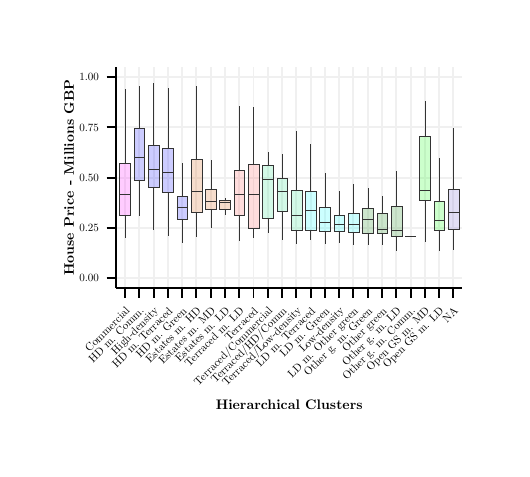
\begin{tikzpicture}[x=1pt,y=1pt]
\definecolor{fillColor}{RGB}{255,255,255}
\path[use as bounding box,fill=fillColor,fill opacity=0.00] (0,0) rectangle (171.17,152.15);
\begin{scope}
\path[clip] (  0.00,  0.00) rectangle (171.17,152.15);
\definecolor{fillColor}{RGB}{255,255,255}

\path[fill=fillColor] (  0.00,  0.00) rectangle (171.17,152.15);
\end{scope}
\begin{scope}
\path[clip] ( 32.06, 58.04) rectangle (156.94,137.92);
\definecolor{fillColor}{RGB}{255,255,255}

\path[fill=fillColor] ( 32.06, 58.04) rectangle (156.94,137.92);
\definecolor{drawColor}{gray}{0.94}

\path[draw=drawColor,line width= 0.7pt,line join=round] ( 32.06, 61.67) --
	(156.94, 61.67);

\path[draw=drawColor,line width= 0.7pt,line join=round] ( 32.06, 79.82) --
	(156.94, 79.82);

\path[draw=drawColor,line width= 0.7pt,line join=round] ( 32.06, 97.98) --
	(156.94, 97.98);

\path[draw=drawColor,line width= 0.7pt,line join=round] ( 32.06,116.13) --
	(156.94,116.13);

\path[draw=drawColor,line width= 0.7pt,line join=round] ( 32.06,134.29) --
	(156.94,134.29);

\path[draw=drawColor,line width= 0.7pt,line join=round] ( 35.15, 58.04) --
	( 35.15,137.92);

\path[draw=drawColor,line width= 0.7pt,line join=round] ( 40.31, 58.04) --
	( 40.31,137.92);

\path[draw=drawColor,line width= 0.7pt,line join=round] ( 45.48, 58.04) --
	( 45.48,137.92);

\path[draw=drawColor,line width= 0.7pt,line join=round] ( 50.64, 58.04) --
	( 50.64,137.92);

\path[draw=drawColor,line width= 0.7pt,line join=round] ( 55.80, 58.04) --
	( 55.80,137.92);

\path[draw=drawColor,line width= 0.7pt,line join=round] ( 60.96, 58.04) --
	( 60.96,137.92);

\path[draw=drawColor,line width= 0.7pt,line join=round] ( 66.12, 58.04) --
	( 66.12,137.92);

\path[draw=drawColor,line width= 0.7pt,line join=round] ( 71.28, 58.04) --
	( 71.28,137.92);

\path[draw=drawColor,line width= 0.7pt,line join=round] ( 76.44, 58.04) --
	( 76.44,137.92);

\path[draw=drawColor,line width= 0.7pt,line join=round] ( 81.60, 58.04) --
	( 81.60,137.92);

\path[draw=drawColor,line width= 0.7pt,line join=round] ( 86.76, 58.04) --
	( 86.76,137.92);

\path[draw=drawColor,line width= 0.7pt,line join=round] ( 91.92, 58.04) --
	( 91.92,137.92);

\path[draw=drawColor,line width= 0.7pt,line join=round] ( 97.08, 58.04) --
	( 97.08,137.92);

\path[draw=drawColor,line width= 0.7pt,line join=round] (102.24, 58.04) --
	(102.24,137.92);

\path[draw=drawColor,line width= 0.7pt,line join=round] (107.40, 58.04) --
	(107.40,137.92);

\path[draw=drawColor,line width= 0.7pt,line join=round] (112.56, 58.04) --
	(112.56,137.92);

\path[draw=drawColor,line width= 0.7pt,line join=round] (117.72, 58.04) --
	(117.72,137.92);

\path[draw=drawColor,line width= 0.7pt,line join=round] (122.88, 58.04) --
	(122.88,137.92);

\path[draw=drawColor,line width= 0.7pt,line join=round] (128.04, 58.04) --
	(128.04,137.92);

\path[draw=drawColor,line width= 0.7pt,line join=round] (133.20, 58.04) --
	(133.20,137.92);

\path[draw=drawColor,line width= 0.7pt,line join=round] (138.36, 58.04) --
	(138.36,137.92);

\path[draw=drawColor,line width= 0.7pt,line join=round] (143.52, 58.04) --
	(143.52,137.92);

\path[draw=drawColor,line width= 0.7pt,line join=round] (148.68, 58.04) --
	(148.68,137.92);

\path[draw=drawColor,line width= 0.7pt,line join=round] (153.84, 58.04) --
	(153.84,137.92);
\definecolor{drawColor}{gray}{0.20}

\path[draw=drawColor,line width= 0.1pt,line join=round] ( 40.31,115.98) -- ( 40.31,131.23);

\path[draw=drawColor,line width= 0.1pt,line join=round] ( 40.31, 97.07) -- ( 40.31, 84.24);
\definecolor{fillColor}{RGB}{0,0,255}

\path[draw=drawColor,line width= 0.1pt,fill=fillColor,fill opacity=0.20] ( 38.38,115.98) --
	( 38.38, 97.07) --
	( 42.25, 97.07) --
	( 42.25,115.98) --
	( 38.38,115.98) --
	cycle;

\path[draw=drawColor,line width= 0.1pt] ( 38.38,105.36) -- ( 42.25,105.36);

\path[draw=drawColor,line width= 0.1pt,line join=round] ( 45.48,109.61) -- ( 45.48,132.25);

\path[draw=drawColor,line width= 0.1pt,line join=round] ( 45.48, 94.50) -- ( 45.48, 79.05);

\path[draw=drawColor,line width= 0.1pt,fill=fillColor,fill opacity=0.20] ( 43.54,109.61) --
	( 43.54, 94.50) --
	( 47.41, 94.50) --
	( 47.41,109.61) --
	( 43.54,109.61) --
	cycle;

\path[draw=drawColor,line width= 0.1pt] ( 43.54,101.01) -- ( 47.41,101.01);

\path[draw=drawColor,line width= 0.1pt,line join=round] ( 35.15,103.32) -- ( 35.15,129.97);

\path[draw=drawColor,line width= 0.1pt,line join=round] ( 35.15, 84.55) -- ( 35.15, 76.26);
\definecolor{fillColor}{RGB}{255,0,255}

\path[draw=drawColor,line width= 0.1pt,fill=fillColor,fill opacity=0.20] ( 33.22,103.32) --
	( 33.22, 84.55) --
	( 37.09, 84.55) --
	( 37.09,103.32) --
	( 33.22,103.32) --
	cycle;

\path[draw=drawColor,line width= 0.1pt] ( 33.22, 91.86) -- ( 37.09, 91.86);

\path[draw=drawColor,line width= 0.1pt,line join=round] (102.24, 93.26) -- (102.24,110.12);

\path[draw=drawColor,line width= 0.1pt,line join=round] (102.24, 79.16) -- (102.24, 75.32);
\definecolor{fillColor}{RGB}{0,255,255}

\path[draw=drawColor,line width= 0.1pt,fill=fillColor,fill opacity=0.20] (100.30, 93.26) --
	(100.30, 79.16) --
	(104.17, 79.16) --
	(104.17, 93.26) --
	(100.30, 93.26) --
	cycle;

\path[draw=drawColor,line width= 0.1pt] (100.30, 86.08) -- (104.17, 86.08);

\path[draw=drawColor,line width= 0.1pt,line join=round] (107.40, 87.19) -- (107.40, 99.76);

\path[draw=drawColor,line width= 0.1pt,line join=round] (107.40, 78.52) -- (107.40, 73.83);

\path[draw=drawColor,line width= 0.1pt,fill=fillColor,fill opacity=0.20] (105.46, 87.19) --
	(105.46, 78.52) --
	(109.33, 78.52) --
	(109.33, 87.19) --
	(105.46, 87.19) --
	cycle;

\path[draw=drawColor,line width= 0.1pt] (105.46, 81.90) -- (109.33, 81.90);

\path[draw=drawColor,line width= 0.1pt,line join=round] (133.20, 87.69) -- (133.20,100.43);

\path[draw=drawColor,line width= 0.1pt,line join=round] (133.20, 76.64) -- (133.20, 71.47);
\definecolor{fillColor}{RGB}{0,128,0}

\path[draw=drawColor,line width= 0.1pt,fill=fillColor,fill opacity=0.20] (131.27, 87.69) --
	(131.27, 76.64) --
	(135.14, 76.64) --
	(135.14, 87.69) --
	(131.27, 87.69) --
	cycle;

\path[draw=drawColor,line width= 0.1pt] (131.27, 78.94) -- (135.14, 78.94);

\path[draw=drawColor,line width= 0.1pt,line join=round] ( 76.44,100.51) -- ( 76.44,123.69);

\path[draw=drawColor,line width= 0.1pt,line join=round] ( 76.44, 84.23) -- ( 76.44, 75.16);
\definecolor{fillColor}{RGB}{255,85,85}

\path[draw=drawColor,line width= 0.1pt,fill=fillColor,fill opacity=0.20] ( 74.50,100.51) --
	( 74.50, 84.23) --
	( 78.37, 84.23) --
	( 78.37,100.51) --
	( 74.50,100.51) --
	cycle;

\path[draw=drawColor,line width= 0.1pt] ( 74.50, 91.91) -- ( 78.37, 91.91);

\path[draw=drawColor,line width= 0.1pt,line join=round] ( 55.80, 91.44) -- ( 55.80,103.24);

\path[draw=drawColor,line width= 0.1pt,line join=round] ( 55.80, 83.10) -- ( 55.80, 74.44);
\definecolor{fillColor}{RGB}{0,0,255}

\path[draw=drawColor,line width= 0.1pt,fill=fillColor,fill opacity=0.20] ( 53.86, 91.44) --
	( 53.86, 83.10) --
	( 57.73, 83.10) --
	( 57.73, 91.44) --
	( 53.86, 91.44) --
	cycle;

\path[draw=drawColor,line width= 0.1pt] ( 53.86, 87.12) -- ( 57.73, 87.12);

\path[draw=drawColor,line width= 0.1pt,line join=round] ( 81.60,102.73) -- ( 81.60,123.65);

\path[draw=drawColor,line width= 0.1pt,line join=round] ( 81.60, 79.60) -- ( 81.60, 76.32);
\definecolor{fillColor}{RGB}{255,85,85}

\path[draw=drawColor,line width= 0.1pt,fill=fillColor,fill opacity=0.20] ( 79.66,102.73) --
	( 79.66, 79.60) --
	( 83.53, 79.60) --
	( 83.53,102.73) --
	( 79.66,102.73) --
	cycle;

\path[draw=drawColor,line width= 0.1pt] ( 79.66, 91.83) -- ( 83.53, 91.83);

\path[draw=drawColor,line width= 0.1pt,line join=round] ( 50.64,108.62) -- ( 50.64,130.37);

\path[draw=drawColor,line width= 0.1pt,line join=round] ( 50.64, 92.61) -- ( 50.64, 76.77);
\definecolor{fillColor}{RGB}{0,0,255}

\path[draw=drawColor,line width= 0.1pt,fill=fillColor,fill opacity=0.20] ( 48.70,108.62) --
	( 48.70, 92.61) --
	( 52.57, 92.61) --
	( 52.57,108.62) --
	( 48.70,108.62) --
	cycle;

\path[draw=drawColor,line width= 0.1pt] ( 48.70, 99.89) -- ( 52.57, 99.89);

\path[draw=drawColor,line width= 0.1pt,line join=round] (117.72, 85.17) -- (117.72, 95.58);

\path[draw=drawColor,line width= 0.1pt,line join=round] (117.72, 78.13) -- (117.72, 73.60);
\definecolor{fillColor}{RGB}{0,255,255}

\path[draw=drawColor,line width= 0.1pt,fill=fillColor,fill opacity=0.20] (115.79, 85.17) --
	(115.79, 78.13) --
	(119.66, 78.13) --
	(119.66, 85.17) --
	(115.79, 85.17) --
	cycle;

\path[draw=drawColor,line width= 0.1pt] (115.79, 81.06) -- (119.66, 81.06);

\path[draw=drawColor,line width= 0.1pt,line join=round] (112.56, 84.35) -- (112.56, 92.98);

\path[draw=drawColor,line width= 0.1pt,line join=round] (112.56, 78.55) -- (112.56, 74.34);

\path[draw=drawColor,line width= 0.1pt,fill=fillColor,fill opacity=0.20] (110.62, 84.35) --
	(110.62, 78.55) --
	(114.50, 78.55) --
	(114.50, 84.35) --
	(110.62, 84.35) --
	cycle;

\path[draw=drawColor,line width= 0.1pt] (110.62, 81.07) -- (114.50, 81.07);

\path[draw=drawColor,line width= 0.1pt,line join=round] (128.04, 84.98) -- (128.04, 91.23);

\path[draw=drawColor,line width= 0.1pt,line join=round] (128.04, 77.76) -- (128.04, 73.79);
\definecolor{fillColor}{RGB}{0,128,0}

\path[draw=drawColor,line width= 0.1pt,fill=fillColor,fill opacity=0.20] (126.11, 84.98) --
	(126.11, 77.76) --
	(129.98, 77.76) --
	(129.98, 84.98) --
	(126.11, 84.98) --
	cycle;

\path[draw=drawColor,line width= 0.1pt] (126.11, 79.46) -- (129.98, 79.46);

\path[draw=drawColor,line width= 0.1pt,line join=round] (122.88, 87.00) -- (122.88, 94.06);

\path[draw=drawColor,line width= 0.1pt,line join=round] (122.88, 77.94) -- (122.88, 73.53);

\path[draw=drawColor,line width= 0.1pt,fill=fillColor,fill opacity=0.20] (120.95, 87.00) --
	(120.95, 77.94) --
	(124.82, 77.94) --
	(124.82, 87.00) --
	(120.95, 87.00) --
	cycle;

\path[draw=drawColor,line width= 0.1pt] (120.95, 82.93) -- (124.82, 82.93);

\path[draw=drawColor,line width= 0.1pt,line join=round] ( 97.08, 93.60) -- ( 97.08,114.66);

\path[draw=drawColor,line width= 0.1pt,line join=round] ( 97.08, 79.07) -- ( 97.08, 73.80);
\definecolor{fillColor}{RGB}{37,229,137}

\path[draw=drawColor,line width= 0.1pt,fill=fillColor,fill opacity=0.20] ( 95.14, 93.60) --
	( 95.14, 79.07) --
	( 99.01, 79.07) --
	( 99.01, 93.60) --
	( 95.14, 93.60) --
	cycle;

\path[draw=drawColor,line width= 0.1pt] ( 95.14, 84.57) -- ( 99.01, 84.57);

\path[draw=drawColor,line width= 0.1pt,line join=round] (148.68, 89.40) -- (148.68,104.95);

\path[draw=drawColor,line width= 0.1pt,line join=round] (148.68, 78.98) -- (148.68, 71.36);
\definecolor{fillColor}{RGB}{0,255,0}

\path[draw=drawColor,line width= 0.1pt,fill=fillColor,fill opacity=0.20] (146.75, 89.40) --
	(146.75, 78.98) --
	(150.62, 78.98) --
	(150.62, 89.40) --
	(146.75, 89.40) --
	cycle;

\path[draw=drawColor,line width= 0.1pt] (146.75, 82.61) -- (150.62, 82.61);

\path[draw=drawColor,line width= 0.1pt,line join=round] ( 91.92, 97.68) -- ( 91.92,106.44);

\path[draw=drawColor,line width= 0.1pt,line join=round] ( 91.92, 86.02) -- ( 91.92, 75.52);
\definecolor{fillColor}{RGB}{37,229,137}

\path[draw=drawColor,line width= 0.1pt,fill=fillColor,fill opacity=0.20] ( 89.98, 97.68) --
	( 89.98, 86.02) --
	( 93.85, 86.02) --
	( 93.85, 97.68) --
	( 89.98, 97.68) --
	cycle;

\path[draw=drawColor,line width= 0.1pt] ( 89.98, 93.17) -- ( 93.85, 93.17);

\path[draw=drawColor,line width= 0.1pt,line join=round] ( 60.96,104.82) -- ( 60.96,131.08);

\path[draw=drawColor,line width= 0.1pt,line join=round] ( 60.96, 85.44) -- ( 60.96, 76.38);
\definecolor{fillColor}{RGB}{212,85,0}

\path[draw=drawColor,line width= 0.1pt,fill=fillColor,fill opacity=0.20] ( 59.02,104.82) --
	( 59.02, 85.44) --
	( 62.89, 85.44) --
	( 62.89,104.82) --
	( 59.02,104.82) --
	cycle;

\path[draw=drawColor,line width= 0.1pt] ( 59.02, 93.21) -- ( 62.89, 93.21);

\path[draw=drawColor,line width= 0.1pt,line join=round] (143.52,112.82) -- (143.52,125.78);

\path[draw=drawColor,line width= 0.1pt,line join=round] (143.52, 89.85) -- (143.52, 74.61);
\definecolor{fillColor}{RGB}{0,255,0}

\path[draw=drawColor,line width= 0.1pt,fill=fillColor,fill opacity=0.20] (141.59,112.82) --
	(141.59, 89.85) --
	(145.46, 89.85) --
	(145.46,112.82) --
	(141.59,112.82) --
	cycle;

\path[draw=drawColor,line width= 0.1pt] (141.59, 93.52) -- (145.46, 93.52);

\path[draw=drawColor,line width= 0.1pt,line join=round] ( 86.76,102.36) -- ( 86.76,107.05);

\path[draw=drawColor,line width= 0.1pt,line join=round] ( 86.76, 83.35) -- ( 86.76, 78.05);
\definecolor{fillColor}{RGB}{37,229,137}

\path[draw=drawColor,line width= 0.1pt,fill=fillColor,fill opacity=0.20] ( 84.82,102.36) --
	( 84.82, 83.35) --
	( 88.69, 83.35) --
	( 88.69,102.36) --
	( 84.82,102.36) --
	cycle;

\path[draw=drawColor,line width= 0.1pt] ( 84.82, 97.46) -- ( 88.69, 97.46);

\path[draw=drawColor,line width= 0.1pt,line join=round] ( 66.12, 93.75) -- ( 66.12,104.36);

\path[draw=drawColor,line width= 0.1pt,line join=round] ( 66.12, 86.41) -- ( 66.12, 79.80);
\definecolor{fillColor}{RGB}{212,85,0}

\path[draw=drawColor,line width= 0.1pt,fill=fillColor,fill opacity=0.20] ( 64.18, 93.75) --
	( 64.18, 86.41) --
	( 68.05, 86.41) --
	( 68.05, 93.75) --
	( 64.18, 93.75) --
	cycle;

\path[draw=drawColor,line width= 0.1pt] ( 64.18, 89.36) -- ( 68.05, 89.36);

\path[draw=drawColor,line width= 0.1pt,line join=round] ( 71.28, 89.91) -- ( 71.28, 90.75);

\path[draw=drawColor,line width= 0.1pt,line join=round] ( 71.28, 86.46) -- ( 71.28, 84.29);

\path[draw=drawColor,line width= 0.1pt,fill=fillColor,fill opacity=0.20] ( 69.34, 89.91) --
	( 69.34, 86.46) --
	( 73.21, 86.46) --
	( 73.21, 89.91) --
	( 69.34, 89.91) --
	cycle;

\path[draw=drawColor,line width= 0.1pt] ( 69.34, 88.94) -- ( 73.21, 88.94);

\path[draw=drawColor,line width= 0.1pt,line join=round] (138.36, 76.92) -- (138.36, 76.92);

\path[draw=drawColor,line width= 0.1pt,line join=round] (138.36, 76.92) -- (138.36, 76.92);
\definecolor{fillColor}{RGB}{0,128,0}

\path[draw=drawColor,line width= 0.1pt,fill=fillColor,fill opacity=0.20] (136.43, 76.92) --
	(136.43, 76.92) --
	(140.30, 76.92) --
	(140.30, 76.92) --
	(136.43, 76.92) --
	cycle;

\path[draw=drawColor,line width= 0.1pt] (136.43, 76.92) -- (140.30, 76.92);

\path[draw=drawColor,line width= 0.1pt,line join=round] (153.84, 93.95) -- (153.84,116.05);

\path[draw=drawColor,line width= 0.1pt,line join=round] (153.84, 79.21) -- (153.84, 71.79);
\definecolor{fillColor}{RGB}{106,90,205}

\path[draw=drawColor,line width= 0.1pt,fill=fillColor,fill opacity=0.20] (151.91, 93.95) --
	(151.91, 79.21) --
	(155.78, 79.21) --
	(155.78, 93.95) --
	(151.91, 93.95) --
	cycle;

\path[draw=drawColor,line width= 0.1pt] (151.91, 85.48) -- (155.78, 85.48);

\path[] ( 32.06, 58.04) rectangle (156.94,137.92);
\end{scope}
\begin{scope}
\path[clip] (  0.00,  0.00) rectangle (171.17,152.15);
\definecolor{drawColor}{RGB}{0,0,0}

\path[draw=drawColor,line width= 0.7pt,line join=round] ( 32.06, 58.04) --
	( 32.06,137.92);
\end{scope}
\begin{scope}
\path[clip] (  0.00,  0.00) rectangle (171.17,152.15);
\definecolor{drawColor}{RGB}{0,0,0}

\node[text=drawColor,anchor=base east,inner sep=0pt, outer sep=0pt, scale=  0.40] at ( 25.76, 60.29) {0.00};

\node[text=drawColor,anchor=base east,inner sep=0pt, outer sep=0pt, scale=  0.40] at ( 25.76, 78.45) {0.25};

\node[text=drawColor,anchor=base east,inner sep=0pt, outer sep=0pt, scale=  0.40] at ( 25.76, 96.60) {0.50};

\node[text=drawColor,anchor=base east,inner sep=0pt, outer sep=0pt, scale=  0.40] at ( 25.76,114.76) {0.75};

\node[text=drawColor,anchor=base east,inner sep=0pt, outer sep=0pt, scale=  0.40] at ( 25.76,132.91) {1.00};
\end{scope}
\begin{scope}
\path[clip] (  0.00,  0.00) rectangle (171.17,152.15);
\definecolor{drawColor}{RGB}{0,0,0}

\path[draw=drawColor,line width= 0.7pt,line join=round] ( 28.56, 61.67) --
	( 32.06, 61.67);

\path[draw=drawColor,line width= 0.7pt,line join=round] ( 28.56, 79.82) --
	( 32.06, 79.82);

\path[draw=drawColor,line width= 0.7pt,line join=round] ( 28.56, 97.98) --
	( 32.06, 97.98);

\path[draw=drawColor,line width= 0.7pt,line join=round] ( 28.56,116.13) --
	( 32.06,116.13);

\path[draw=drawColor,line width= 0.7pt,line join=round] ( 28.56,134.29) --
	( 32.06,134.29);
\end{scope}
\begin{scope}
\path[clip] (  0.00,  0.00) rectangle (171.17,152.15);
\definecolor{drawColor}{RGB}{0,0,0}

\path[draw=drawColor,line width= 0.7pt,line join=round] ( 32.06, 58.04) --
	(156.94, 58.04);
\end{scope}
\begin{scope}
\path[clip] (  0.00,  0.00) rectangle (171.17,152.15);
\definecolor{drawColor}{RGB}{0,0,0}

\path[draw=drawColor,line width= 0.7pt,line join=round] ( 35.15, 54.54) --
	( 35.15, 58.04);

\path[draw=drawColor,line width= 0.7pt,line join=round] ( 40.31, 54.54) --
	( 40.31, 58.04);

\path[draw=drawColor,line width= 0.7pt,line join=round] ( 45.48, 54.54) --
	( 45.48, 58.04);

\path[draw=drawColor,line width= 0.7pt,line join=round] ( 50.64, 54.54) --
	( 50.64, 58.04);

\path[draw=drawColor,line width= 0.7pt,line join=round] ( 55.80, 54.54) --
	( 55.80, 58.04);

\path[draw=drawColor,line width= 0.7pt,line join=round] ( 60.96, 54.54) --
	( 60.96, 58.04);

\path[draw=drawColor,line width= 0.7pt,line join=round] ( 66.12, 54.54) --
	( 66.12, 58.04);

\path[draw=drawColor,line width= 0.7pt,line join=round] ( 71.28, 54.54) --
	( 71.28, 58.04);

\path[draw=drawColor,line width= 0.7pt,line join=round] ( 76.44, 54.54) --
	( 76.44, 58.04);

\path[draw=drawColor,line width= 0.7pt,line join=round] ( 81.60, 54.54) --
	( 81.60, 58.04);

\path[draw=drawColor,line width= 0.7pt,line join=round] ( 86.76, 54.54) --
	( 86.76, 58.04);

\path[draw=drawColor,line width= 0.7pt,line join=round] ( 91.92, 54.54) --
	( 91.92, 58.04);

\path[draw=drawColor,line width= 0.7pt,line join=round] ( 97.08, 54.54) --
	( 97.08, 58.04);

\path[draw=drawColor,line width= 0.7pt,line join=round] (102.24, 54.54) --
	(102.24, 58.04);

\path[draw=drawColor,line width= 0.7pt,line join=round] (107.40, 54.54) --
	(107.40, 58.04);

\path[draw=drawColor,line width= 0.7pt,line join=round] (112.56, 54.54) --
	(112.56, 58.04);

\path[draw=drawColor,line width= 0.7pt,line join=round] (117.72, 54.54) --
	(117.72, 58.04);

\path[draw=drawColor,line width= 0.7pt,line join=round] (122.88, 54.54) --
	(122.88, 58.04);

\path[draw=drawColor,line width= 0.7pt,line join=round] (128.04, 54.54) --
	(128.04, 58.04);

\path[draw=drawColor,line width= 0.7pt,line join=round] (133.20, 54.54) --
	(133.20, 58.04);

\path[draw=drawColor,line width= 0.7pt,line join=round] (138.36, 54.54) --
	(138.36, 58.04);

\path[draw=drawColor,line width= 0.7pt,line join=round] (143.52, 54.54) --
	(143.52, 58.04);

\path[draw=drawColor,line width= 0.7pt,line join=round] (148.68, 54.54) --
	(148.68, 58.04);

\path[draw=drawColor,line width= 0.7pt,line join=round] (153.84, 54.54) --
	(153.84, 58.04);
\end{scope}
\begin{scope}
\path[clip] (  0.00,  0.00) rectangle (171.17,152.15);
\definecolor{drawColor}{RGB}{0,0,0}

\node[text=drawColor,rotate= 45.00,anchor=base east,inner sep=0pt, outer sep=0pt, scale=  0.40] at ( 37.08, 49.51) {Commercial};

\node[text=drawColor,rotate= 45.00,anchor=base east,inner sep=0pt, outer sep=0pt, scale=  0.40] at ( 42.24, 49.51) {HD m. Comm.};

\node[text=drawColor,rotate= 45.00,anchor=base east,inner sep=0pt, outer sep=0pt, scale=  0.40] at ( 47.40, 49.51) {High-density};

\node[text=drawColor,rotate= 45.00,anchor=base east,inner sep=0pt, outer sep=0pt, scale=  0.40] at ( 52.56, 49.51) {HD m. Terraced};

\node[text=drawColor,rotate= 45.00,anchor=base east,inner sep=0pt, outer sep=0pt, scale=  0.40] at ( 57.72, 49.51) {HD m. Green};

\node[text=drawColor,rotate= 45.00,anchor=base east,inner sep=0pt, outer sep=0pt, scale=  0.40] at ( 62.88, 49.51) {Estates m. HD};

\node[text=drawColor,rotate= 45.00,anchor=base east,inner sep=0pt, outer sep=0pt, scale=  0.40] at ( 68.05, 49.51) {Estates m. MD};

\node[text=drawColor,rotate= 45.00,anchor=base east,inner sep=0pt, outer sep=0pt, scale=  0.40] at ( 73.21, 49.51) {Estates m. LD};

\node[text=drawColor,rotate= 45.00,anchor=base east,inner sep=0pt, outer sep=0pt, scale=  0.40] at ( 78.37, 49.51) {Terraced m. LD};

\node[text=drawColor,rotate= 45.00,anchor=base east,inner sep=0pt, outer sep=0pt, scale=  0.40] at ( 83.53, 49.51) {Terraced};

\node[text=drawColor,rotate= 45.00,anchor=base east,inner sep=0pt, outer sep=0pt, scale=  0.40] at ( 88.69, 49.51) {Terraced/Commercial};

\node[text=drawColor,rotate= 45.00,anchor=base east,inner sep=0pt, outer sep=0pt, scale=  0.40] at ( 93.85, 49.51) {Terraced/HD/Comm};

\node[text=drawColor,rotate= 45.00,anchor=base east,inner sep=0pt, outer sep=0pt, scale=  0.40] at ( 99.01, 49.51) {Terraced/Low-density};

\node[text=drawColor,rotate= 45.00,anchor=base east,inner sep=0pt, outer sep=0pt, scale=  0.40] at (104.17, 49.51) {LD m. Terraced};

\node[text=drawColor,rotate= 45.00,anchor=base east,inner sep=0pt, outer sep=0pt, scale=  0.40] at (109.33, 49.51) {LD m. Green};

\node[text=drawColor,rotate= 45.00,anchor=base east,inner sep=0pt, outer sep=0pt, scale=  0.40] at (114.49, 49.51) {Low-density};

\node[text=drawColor,rotate= 45.00,anchor=base east,inner sep=0pt, outer sep=0pt, scale=  0.40] at (119.65, 49.51) {LD m. Other green};

\node[text=drawColor,rotate= 45.00,anchor=base east,inner sep=0pt, outer sep=0pt, scale=  0.40] at (124.81, 49.51) {Other g. m. Green};

\node[text=drawColor,rotate= 45.00,anchor=base east,inner sep=0pt, outer sep=0pt, scale=  0.40] at (129.97, 49.51) {Other green};

\node[text=drawColor,rotate= 45.00,anchor=base east,inner sep=0pt, outer sep=0pt, scale=  0.40] at (135.13, 49.51) {Other g. m. LD};

\node[text=drawColor,rotate= 45.00,anchor=base east,inner sep=0pt, outer sep=0pt, scale=  0.40] at (140.29, 49.51) {Other g. m. Comm.};

\node[text=drawColor,rotate= 45.00,anchor=base east,inner sep=0pt, outer sep=0pt, scale=  0.40] at (145.45, 49.51) {Open GS m. MD};

\node[text=drawColor,rotate= 45.00,anchor=base east,inner sep=0pt, outer sep=0pt, scale=  0.40] at (150.61, 49.51) {Open GS m. LD};

\node[text=drawColor,rotate= 45.00,anchor=base east,inner sep=0pt, outer sep=0pt, scale=  0.40] at (155.77, 49.51) {NA};
\end{scope}
\begin{scope}
\path[clip] (  0.00,  0.00) rectangle (171.17,152.15);
\definecolor{drawColor}{RGB}{0,0,0}

\node[text=drawColor,anchor=base,inner sep=0pt, outer sep=0pt, scale=  0.50] at ( 94.50, 14.03) {\bfseries Hierarchical Clusters};
\end{scope}
\begin{scope}
\path[clip] (  0.00,  0.00) rectangle (171.17,152.15);
\definecolor{drawColor}{RGB}{0,0,0}

\node[text=drawColor,rotate= 90.00,anchor=base,inner sep=0pt, outer sep=0pt, scale=  0.50] at ( 16.70, 97.98) {\bfseries House Price - Millions GBP};
\end{scope}
\end{tikzpicture}
